
\chapter{Software Architecture Design}
\label{chap:software-architecture-design}
<TIP: Describe how you design your application using Unified Modelling
Language (UML). There should be at least two diagrams that describe the
software architecture. You may add additional or remove unnecessary diagrams.
However, there needs to be a coherency between them at the end./>

\section{Domain Model}
\label{section:domain-model}
<TIP: Describe the business concept of your project. Showcase a
domain model that captures the said concept./>

\section{Design Class Diagram}
\label{section:design-class-diagram}
<TIP: Showcase a design class diagram for your project and explain
how it works here. You can group classes into packages or layers to communicate your
design better./>

\section{Sequence Diagram}
\label{section:sequence-diagram}
<TIP: Sequence diagrams describe how the software runs at runtime.
You do not have to create a sequence diagram for every scenario. However,
there should be one for all the main ones./>

<ChatGPT: Creating a sequence diagram for every use case is not
strictly necessary, but it can be a valuable tool in certain situations. Sequence
diagrams are particularly useful for illustrating the interactions between different
components or objects in a system over time, showcasing the flow of messages
or actions between them./>

\section{Artificial Intelligence}
\label{section:artificial-intelligence}
WorkQuest's Personalized Feedback feature uses AI to analyze user activity, provide task-related insights, and offer feedback. It helps improve teamwork and efficiency by giving suggestions based on work patterns.

\begin{itemize}
    \item \textbf{Work Speed Analysis} 
    \\ \textit{Input:} Task completion time, daily work speed trends  
    \\ \textit{Technique:} Time series analysis  
    \\ \textit{Output:} Estimates how much time each type of task takes, helping users manage workloads efficiently  
    \begin{figure}[H]
        \centering
        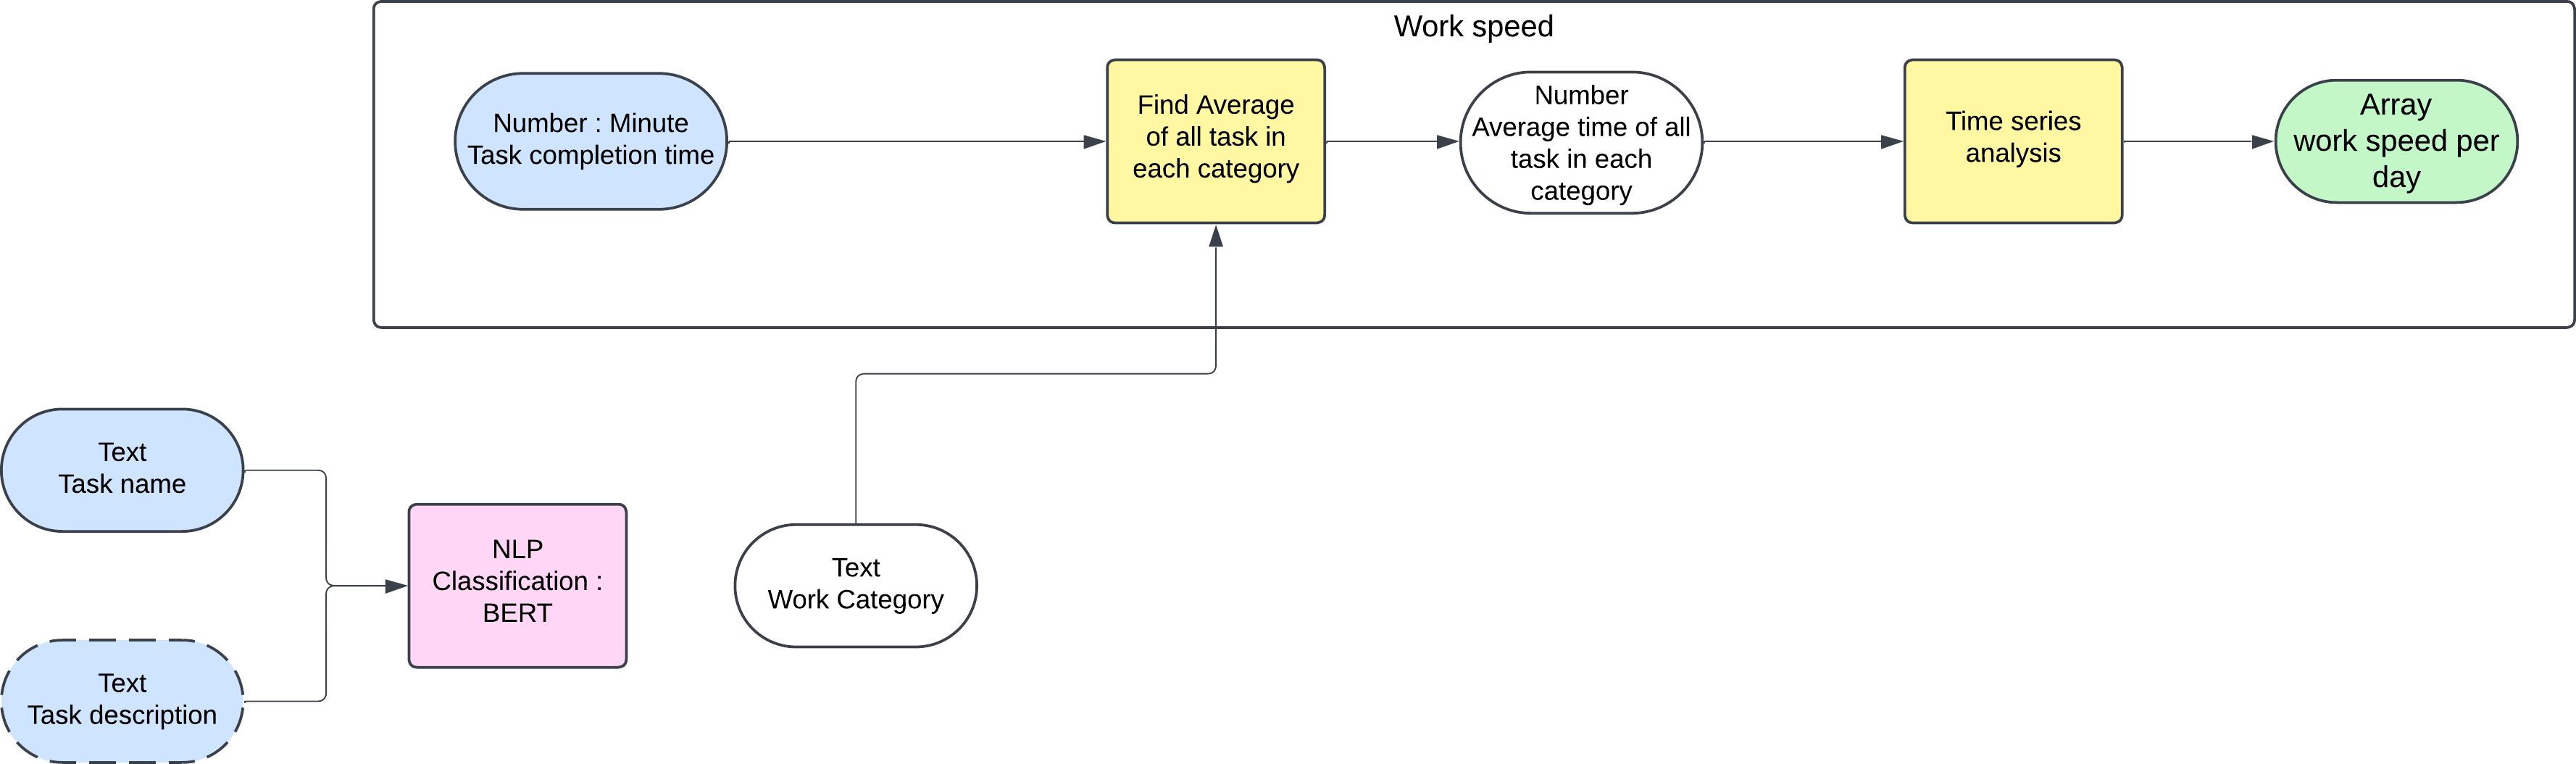
\includegraphics[width=0.6\textwidth]{ai_components/Work_Speed.png}
        \caption{How the AI Component Analyzes Work Speed}
    \end{figure}

    \item \textbf{Strength Identification}  
    \\ \textit{Input:} Task names and descriptions, Work category  
    \\ \textit{Technique:} NLP classification using BERT  
    \\ \textit{Output:} Identifies frequently performed tasks to highlight user strengths  
    \begin{figure}[H]
        \centering
        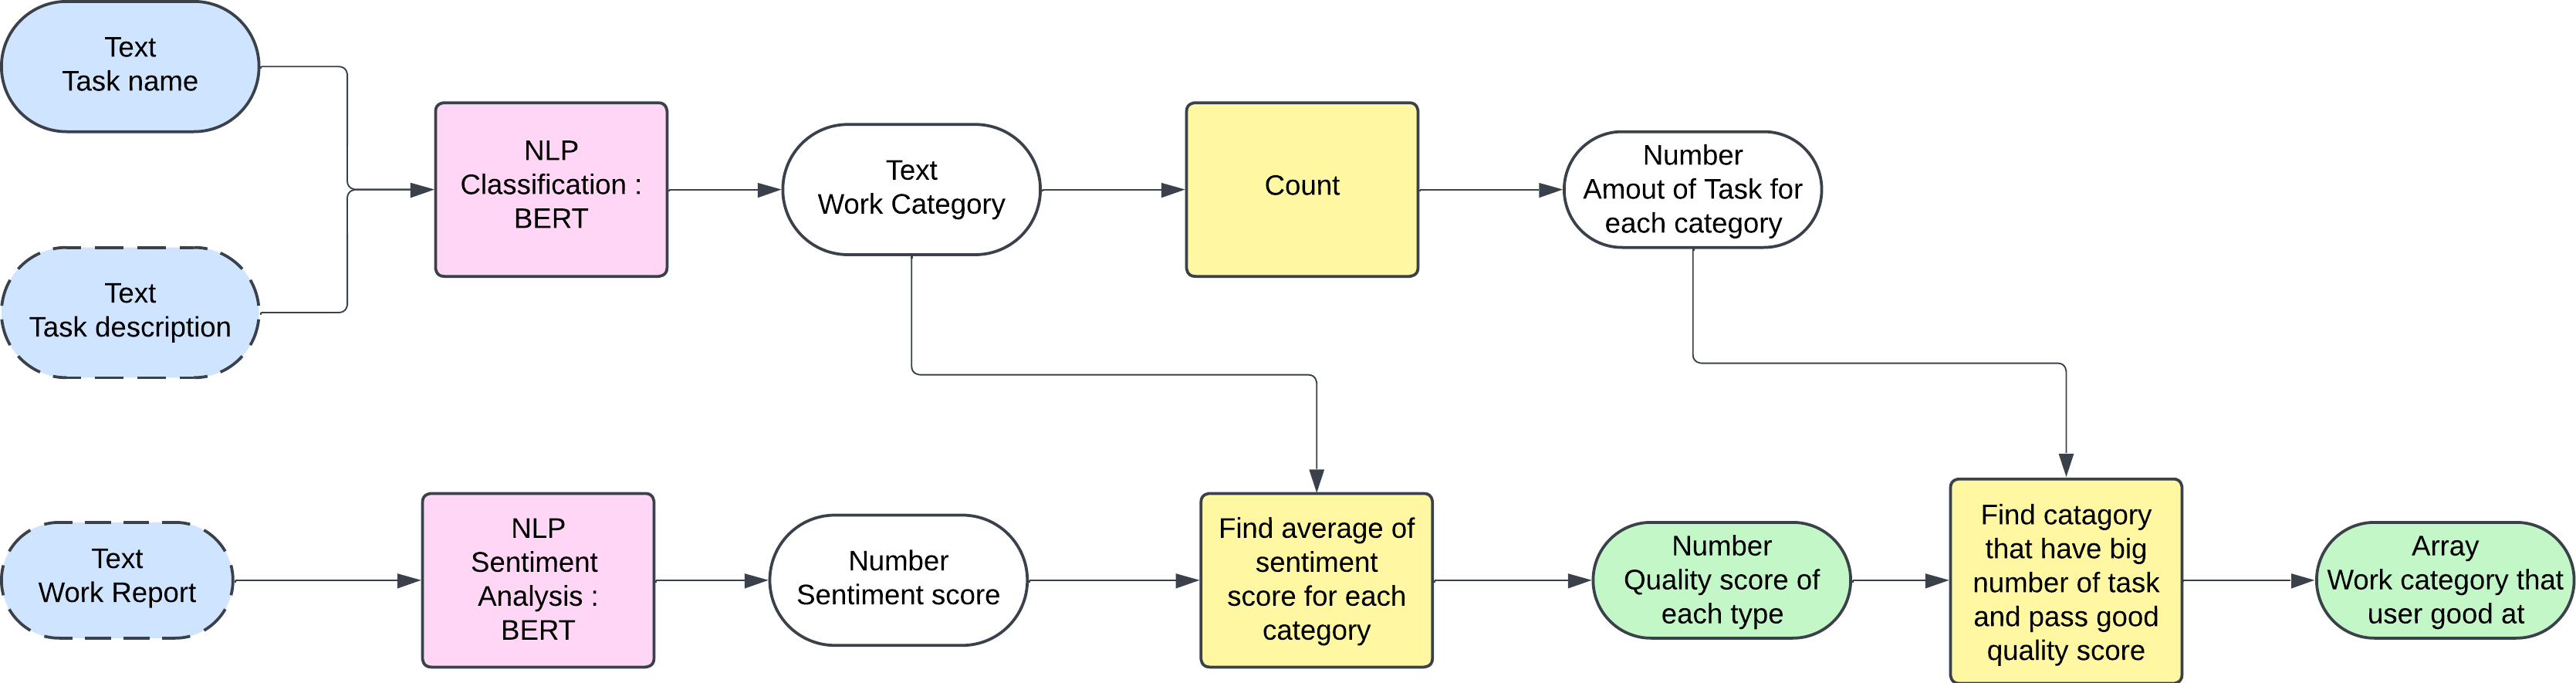
\includegraphics[width=0.6\textwidth]{ai_components/Strenght.png}
        \caption{How the AI Component Identifies Strengths}
    \end{figure}

    \item \textbf{Work Quality Evaluation}  
    \\ \textit{Input:} User-generated work reports and reviews  
    \\ \textit{Technique:} NLP sentiment analysis (RoBERTa)  
    \\ \textit{Output:} Determines whether feedback is positive or negative, influencing motivation and improvement areas  
    \begin{figure}[H]
        \centering
        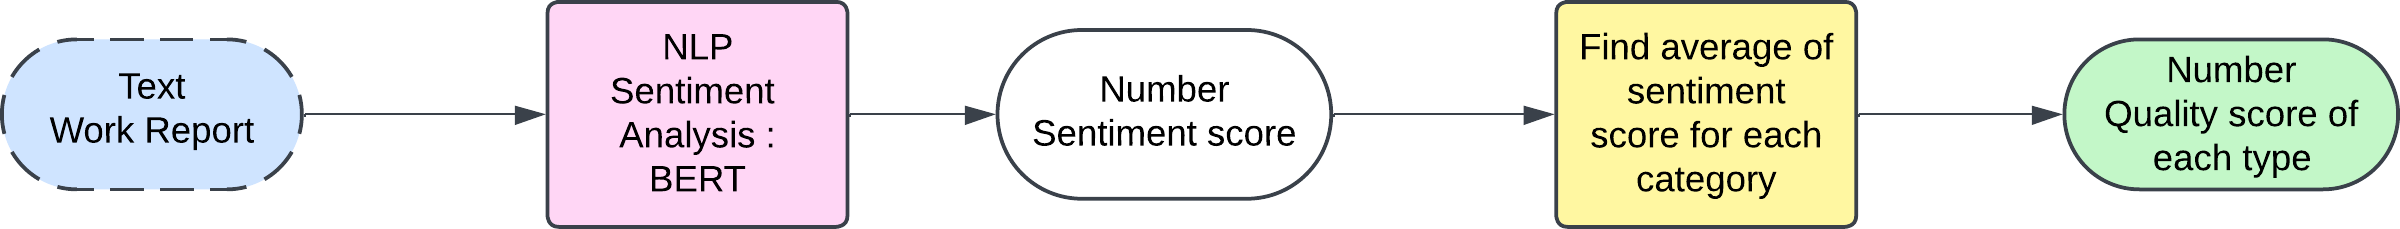
\includegraphics[width=0.6\textwidth]{ai_components/Quality.png}
        \caption{How the AI Component Evaluates Work Quality}
    \end{figure}
   

    \item \textbf{Teamwork Evaluation}  
    \\ \textit{Input:} Number of assigned tasks, teamwork interactions  
    \\ \textit{Technique:} Z-score normalization  
    \\ \textit{Output:} Measures collaboration levels to encourage balanced participation  
    \begin{figure}[H]
        \centering
        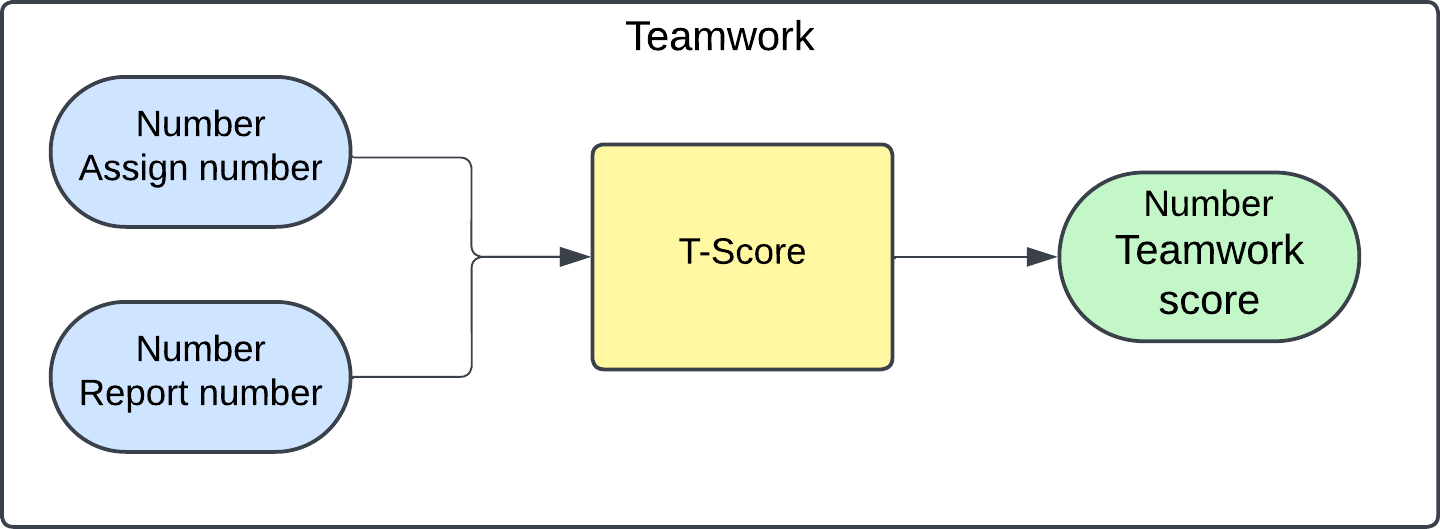
\includegraphics[width=0.6\textwidth]{ai_components/Teamwork.png}
        \caption{How the AI Component Evaluates Teamwork}
    \end{figure}

    \item \textbf{Diligence Scoring}  
    \\ \textit{Input:} Task weight, difficulty level  
    \\ \textit{Technique:} Z-score normalization  
    \\ \textit{Output:} Assesses consistency in handling complex or demanding tasks 
    \begin{figure}[H]
        \centering
        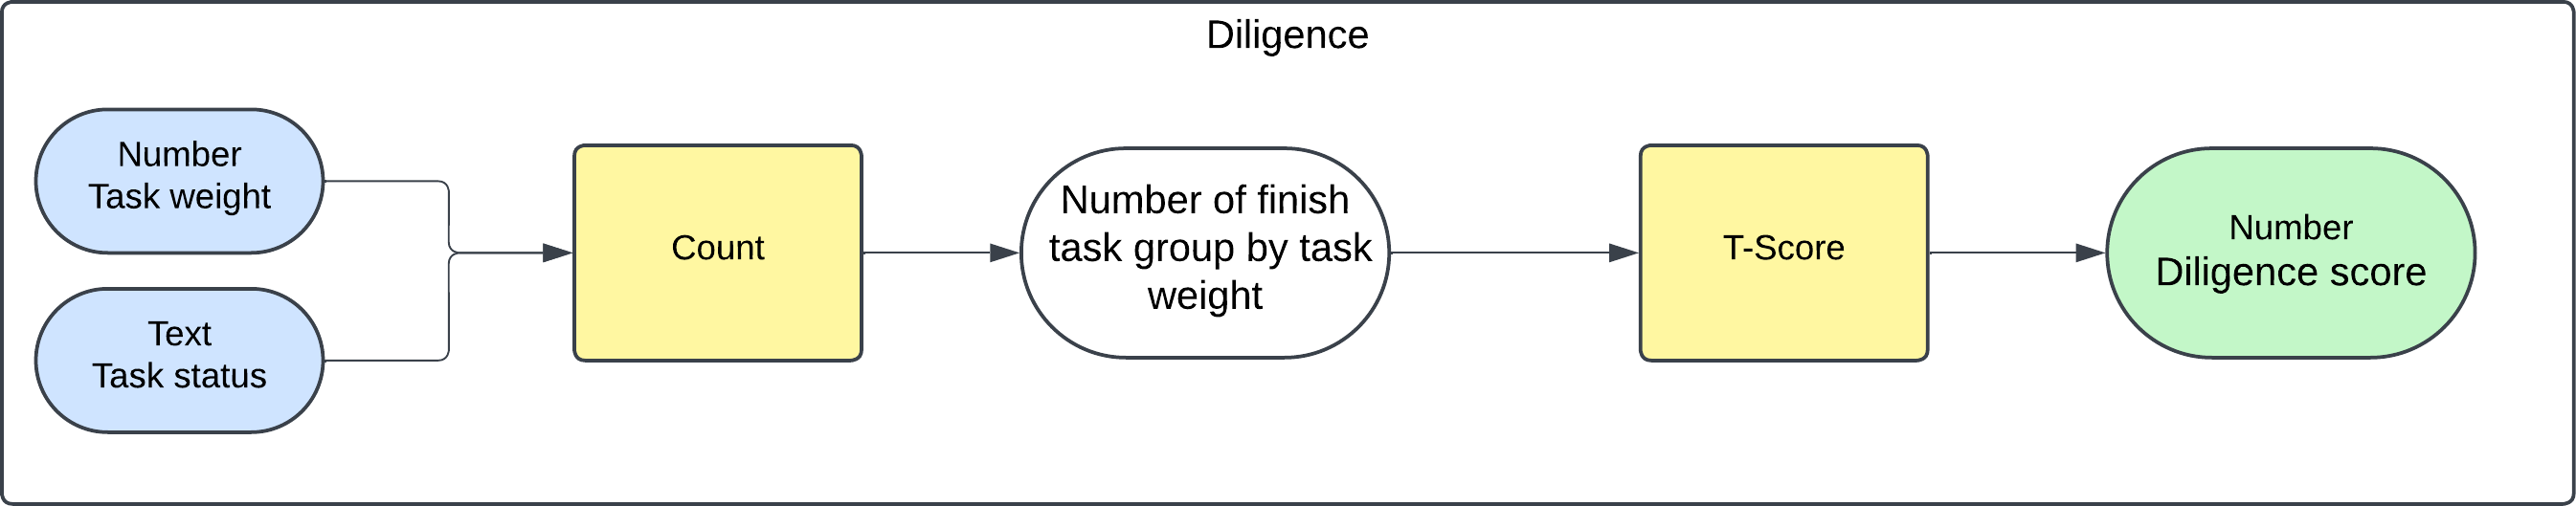
\includegraphics[width=0.6\textwidth]{ai_components/Diligence.png}
        \caption{How the AI Component Evaluates Diligence}
    \end{figure} 

    \item \textbf{Workload Tracking}  
    \\ \textit{Input:} Work session start and end times  
    \\ \textit{Technique:} Time series analysis  
    \\ \textit{Output:} Evaluates work intensity and suggests workload balancing strategies  
    \begin{figure}[H]
        \centering
        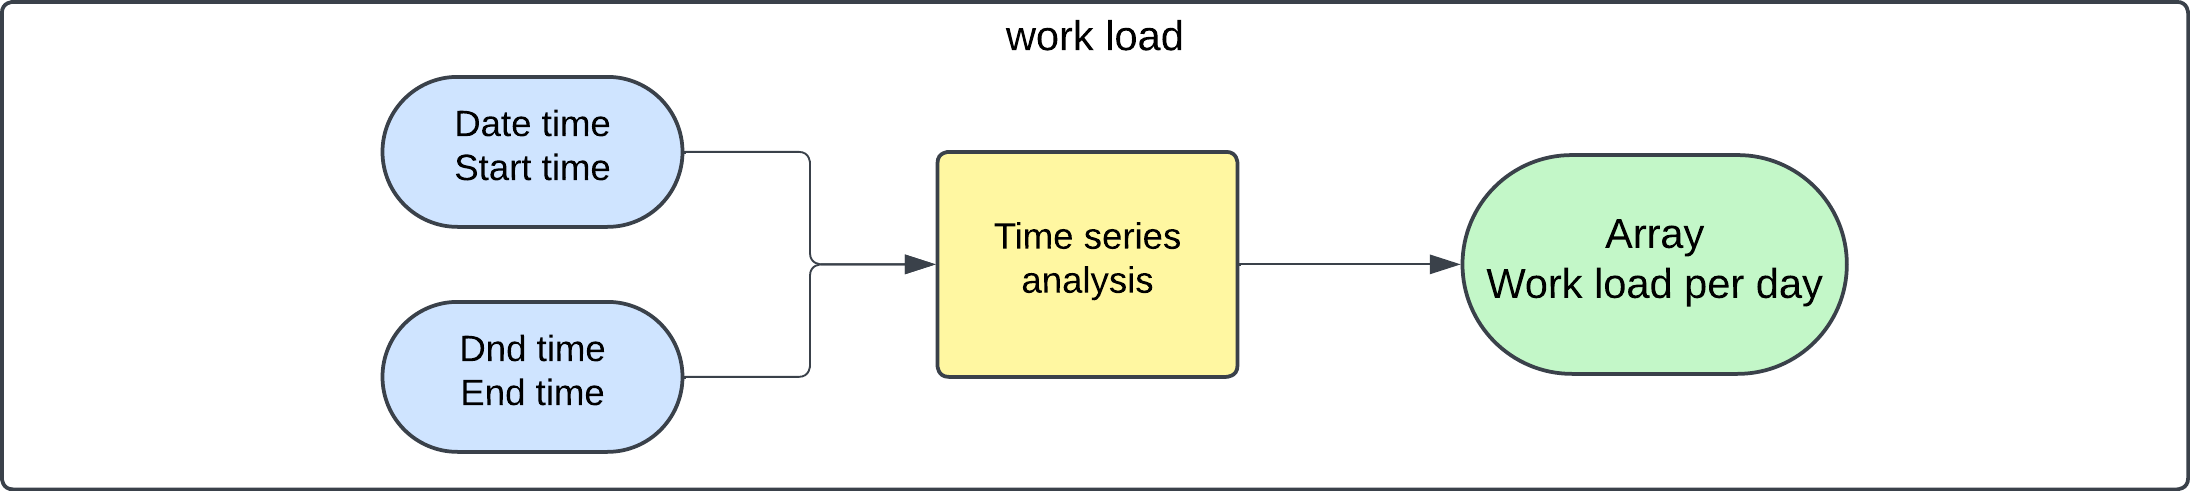
\includegraphics[width=0.6\textwidth]{ai_components/Work_Load.png}
        \caption{How the AI Component Tracks Workload}
    \end{figure}

    \item \textbf{AI-Powered Suggestions} 
    \\ \textit{Technique:} Reinforcement learning (Q-learning)  
    \\ \textit{Output:}  
    \begin{itemize}
        \item \textbf{Prioritization:} Recommends which tasks to focus on  
        \item \textbf{Workload Optimization:} Suggests schedule adjustments to reduce overtime  
        \item \textbf{Collaboration Enhancement:} Identifies opportunities to improve teamwork  
    \end{itemize}
    \begin{figure}[H]
        \centering
        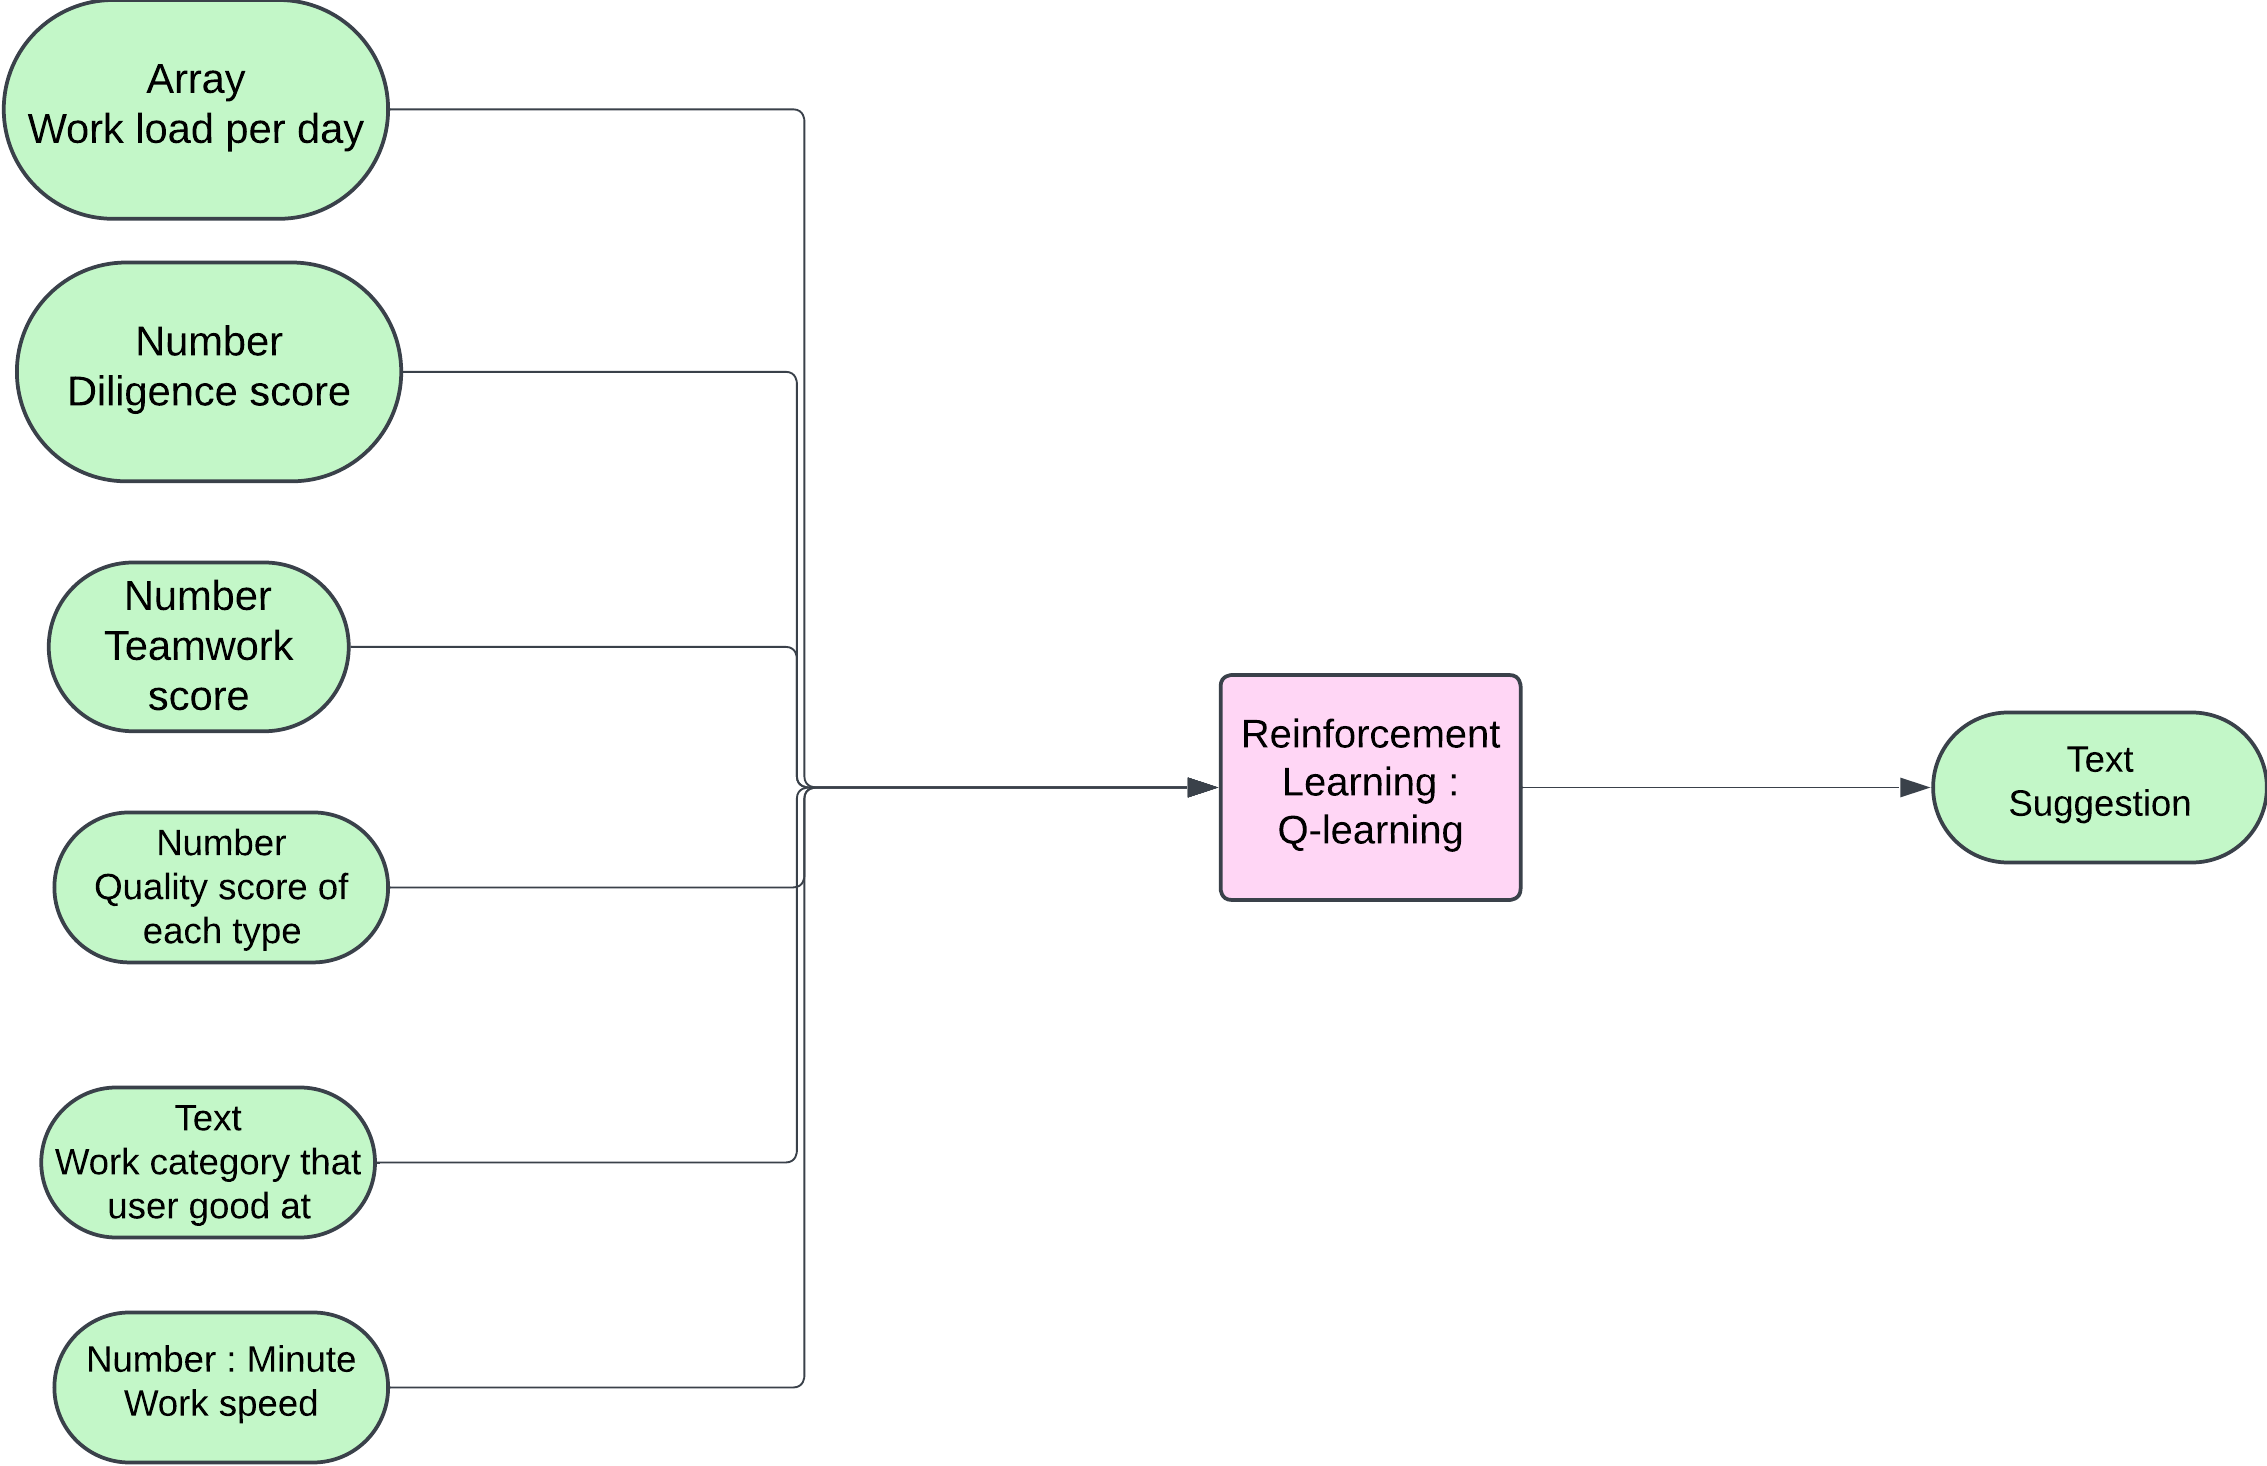
\includegraphics[width=0.6\textwidth]{ai_components/Suggestion.png}
        \caption{How the AI Component Gives Suggestion}
    \end{figure} 

    \item \textbf{Role Categorization}  
    \\ \textit{Input:} Work activity data from all users in the system
    \\ \textit{Technique:} K-Means clustering  
    \\ \textit{Output:} Classifies users into roles based on work habits:  
    % \begin{itemize}
    %     \item \textbf{The Leaders} – Frequently assign tasks and provide feedback  
    %     \item \textbf{The Collaborators} – Actively engage with the team  
    %     \item \textbf{The Quiet Workers} – Prefer working independently  
    %     \item \textbf{The Feedback Experts} – Provide valuable feedback but assign fewer tasks  
    % \end{itemize}
    \textbf{Final Step:} All analyzed outputs from the AI components are processed by OpenAI (GPT) to generate a clear, structured, and user-friendly feedback report.
    
    \subsection{AI Techniques Used}
        \begin{itemize}
            \item \textbf{Natural Language Processing (NLP)}
            \begin{itemize}
                \item \textbf{BERT} – Helps classify tasks and find user strengths.
                \item \textbf{Zero-shot Classification} – Sorts tasks into categories without needing pre-labeled data.
                \item \textbf{Sentiment Analysis (DistilBERT)} – Checks user feedback to understand their opinions.
            \end{itemize}
            
            \item \textbf{Unsupervised Learning}
            \begin{itemize}
                \item \textbf{K-Means Clustering} – Effectively groups users based on performance similarity. As an unsupervised model, it does not require a training dataset.
            \end{itemize}
            
            \item \textbf{Time Series Analysis}  
            \begin{itemize}
                \item Tracks changes in work speed and task load over time.
            \end{itemize}

            \item \textbf{Z-score Normalization}  
            \begin{itemize}
                \item Measures teamwork and effort by comparing user performance.
            \end{itemize}

            \item \textbf{Reinforcement Learning (Q-learning)}  
            \begin{itemize}
                \item Q-learning continuously learns from past actions and rewards, making it effective for task recommendations that improve over time. It can be applied to recommendation scenarios to deliver optimal results.
            \end{itemize}

            \item \textbf{Generative AI (GPT-based Models)}  
            \begin{itemize}
                \item GPT for generating natural language text, making it suitable for turning analytical outputs into understandable and personalized feedback.
            \end{itemize}
        \end{itemize}

    \subsection{Example Usage}
    \textbf{Input:}
    \begin{figure}[H]
        \centering
        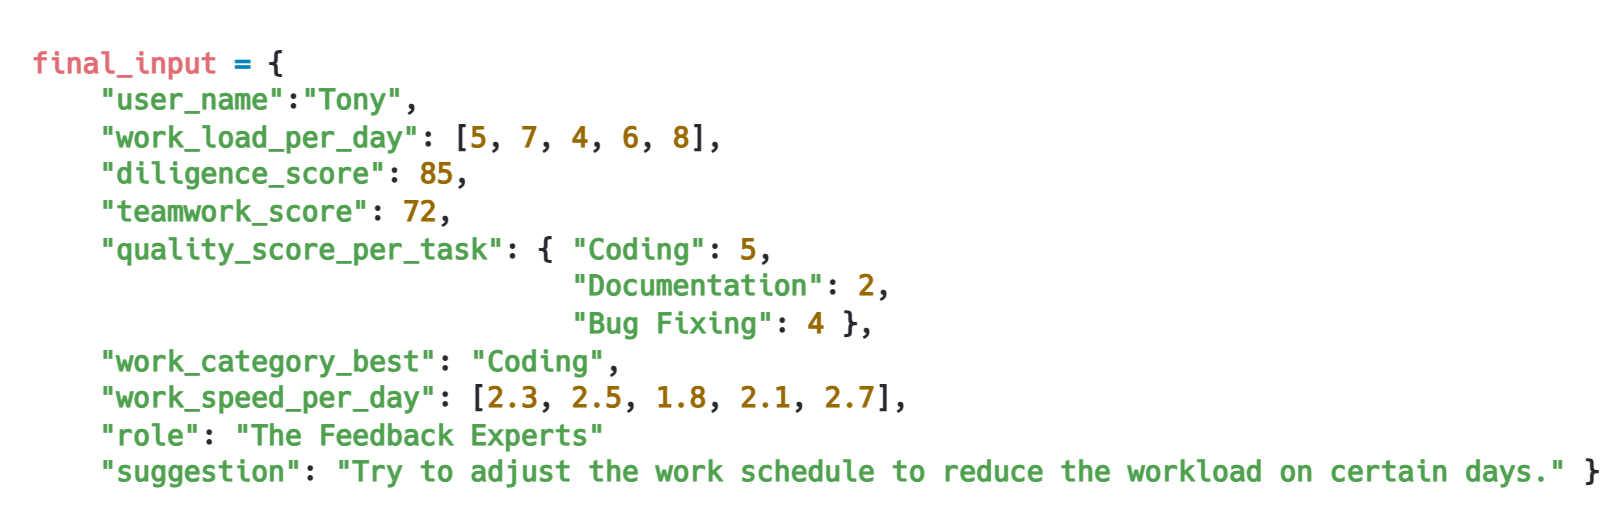
\includegraphics[width=0.9\textwidth]{ai_components/example_input.png}
        \caption{Example input}
    \end{figure}
    \textbf{Output:} \\
     Hey Tony, you're doing great, man! Your coding skills are solid, and you’ve got some seriously strong workdays where you’re super fast. That shows you’ve got the ability to push through when needed. But there are a few things you can level up—teamwork, for example. If you focus a bit more on working smoothly with others, it’ll make a big difference. Also, your documentation and bug fixing are already good, but tightening up the details could make things even sharper. And don’t forget to balance your workload—some days are packed, and that could burn you out. If you manage that better, you’ll be even more efficient and consistent. Keep crushing it! \\
    \textbf{Graphs:}  
    \begin{enumerate}
        \item \textbf{Pie Chart - Review:} Shows the proportion of positive and negative reviews to help understand general sentiment trends.  
        \item \textbf{Bar Chart - Strengths:} Displays tasks that users frequently perform and receive good feedback on, categorized by type. This highlights common areas of positive performance.  
    \end{enumerate}
\end{itemize}

\section{Algorithm}
\label{section:algorithm}
<TIP: Optional, If you are working on a research project that proposes a new
algorithm, you can describe your algorithm here. It can be in the form of
pseudocode or any diagram that you deem appropriate./>